% ===================================================================
%  Week 11 — Session 2: Rectification & Auto-Alignment (RANSAC)
% ===================================================================
\documentclass[10pt,aspectratio=169]{beamer}
% ===================================================================
%  Shared Beamer preamble for "Practical Image Processing"
%  English slides. Compile with pdfLaTeX.
% ===================================================================

\usetheme{metropolis}
\usepackage[T1]{fontenc}
\usepackage[utf8]{inputenc}
\usepackage{lmodern}
\usepackage{listings}
\usepackage{tcolorbox}
\usepackage{fontawesome5}
\usepackage{booktabs}
\usepackage{amsmath,amssymb}
\usepackage{tikz}
\usepackage{pgfplots}
\pgfplotsset{compat=1.17}
\usetikzlibrary{arrows.meta,positioning,shapes.geometric,fit,backgrounds,matrix}
\tcbuselibrary{skins,breakable}

% ---- Palette --------------------------------------------------------
\definecolor{coursePrimary}{HTML}{1B4965}   % deep blue
\definecolor{courseAccent}{HTML}{E76F51}    % coral
\definecolor{courseGood}{HTML}{2A9D8F}      % teal
\definecolor{courseBad}{HTML}{C0392B}       % red
\definecolor{courseInfo}{HTML}{2980B9}      % blue
\definecolor{codeBg}{HTML}{F5F6FA}
\definecolor{codeKw}{HTML}{8E44AD}
\definecolor{codeStr}{HTML}{2A9D8F}
\definecolor{codeCom}{HTML}{7F8C8D}

\setbeamercolor{frametitle}{bg=coursePrimary}
\setbeamercolor{progress bar}{fg=courseAccent}
\setbeamercolor{alerted text}{fg=courseAccent}
\metroset{block=fill,sectionpage=progressbar,numbering=fraction}

% ---- Code listings (Python is built into listings) -----------------
\lstdefinestyle{course}{
  backgroundcolor=\color{codeBg},
  basicstyle=\ttfamily\scriptsize,
  keywordstyle=\color{codeKw}\bfseries,
  stringstyle=\color{codeStr},
  commentstyle=\color{codeCom}\itshape,
  numberstyle=\tiny\color{codeCom},
  numbers=left, numbersep=6pt,
  showstringspaces=false, breaklines=true, breakatwhitespace=true,
  tabsize=4, columns=fullflexible,
  frame=single, framesep=4pt, rulecolor=\color{gray!30},
  keepspaces=true, upquote=true, language=Python,
}
\lstset{style=course}
\lstdefinelanguage{bash}{
  keywords={cd,pip,python,venv,source,import}, sensitive=true,
  morecomment=[l]{\#}, morestring=[b]', morestring=[b]",
}

% ---- Reusable callout boxes ----------------------------------------
\newtcolorbox{goodbox}[1][Good practice]{colback=courseGood!8,colframe=courseGood,
  fonttitle=\bfseries,title={\faCheck~#1},boxrule=0.6pt,left=4pt,right=4pt,top=3pt,bottom=3pt}
\newtcolorbox{badbox}[1][Pitfall]{colback=courseBad!8,colframe=courseBad,
  fonttitle=\bfseries,title={\faTimes~#1},boxrule=0.6pt,left=4pt,right=4pt,top=3pt,bottom=3pt}
\newtcolorbox{infobox}[1][Note]{colback=courseInfo!8,colframe=courseInfo,
  fonttitle=\bfseries,title={\faInfoCircle~#1},boxrule=0.6pt,left=4pt,right=4pt,top=3pt,bottom=3pt}
\newtcolorbox{mathbox}[1][Math]{colback=coursePrimary!6,colframe=coursePrimary,
  fonttitle=\bfseries,title={\faCalculator~#1},boxrule=0.6pt,left=4pt,right=4pt,top=3pt,bottom=3pt}

\newcommand{\keyidea}[1]{\begin{alertblock}{Key idea}#1\end{alertblock}}
\newcommand{\term}[1]{\textbf{\color{coursePrimary}#1}}
\newcommand{\code}[1]{\lstinline[basicstyle=\ttfamily\small]|#1|}

% ---- A helper to draw a small pixel grid, cells shaded by value ----
% \pixelgrid{ {10,20,120,200,240}, {30,60,130,180,230}, ... }
\newcommand{\pixelgrid}[1]{%
  \begin{tikzpicture}[font=\scriptsize,scale=0.6]
    \foreach \row [count=\ry] in {#1} {
      \foreach \val [count=\cx] in \row {
        \draw[gray,fill=coursePrimary!8] (\cx,-\ry) rectangle ++(1,-1);
        \node at (\cx+0.5,-\ry-0.5) {\val};
      }
    }
  \end{tikzpicture}}


\title{Homography \& Perspective Warp}
\subtitle{Week 11 — Session 2: Rectification \& Auto-Alignment (RANSAC)}
\author{Practical Image Processing}
\date{Lecture 11.2 \textbullet\ 60--70 min}

\begin{document}

\maketitle

\begin{frame}{Recap of Session 1}
  \begin{columns}[T]
    \begin{column}{0.56\textwidth}
      \begin{itemize}
        \item Transforms move \emph{positions}; the hierarchy runs rigid $\to$ affine $\to$ projective.
        \item A \term{homography} $H$ is $3\times3$, 8 DoF, defined by \term{4 correspondences}.
        \item Apply it in homogeneous coords, then \emph{divide by $w'$} — the perspective step.
      \end{itemize}
    \end{column}
    \begin{column}{0.44\textwidth}
      \begin{alertblock}{Today: make it a scanner}
        Corners $\to$ destination rectangle $\to$ \code{warpPerspective} $\to$ flat scan, then do it
        \emph{automatically} with matches + RANSAC.
      \end{alertblock}
    \end{column}
  \end{columns}
\end{frame}

\begin{frame}{Roadmap}\tableofcontents\end{frame}

% ==================================================================
\section{Rectification: the DocScan core}
% ==================================================================

\begin{frame}{The rectification idea}
  \begin{enumerate}
    \item Find the 4 corners of the page/meter in the photo (Week 9's \code{approxPolyDP}, or feature matching).
    \item Decide where those corners \emph{should} go: the 4 corners of a clean rectangle.
    \item Compute the homography from photo-corners $\rightarrow$ rectangle-corners.
    \item \code{warpPerspective} the photo through it: out comes a flat, front-on scan.
  \end{enumerate}
  \keyidea{Rectification is just ``I know where these 4 points \emph{should} land'' turned into a warp.}
\end{frame}

\begin{frame}{Step 1--2: a tilted meter and its 4 corners}
  \begin{columns}[T]
    \begin{column}{0.5\textwidth}\begin{center}
      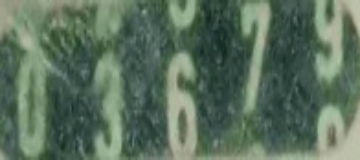
\includegraphics[width=0.95\linewidth]{../assets/original.png}\\{\scriptsize the clean template (target)}
    \end{center}\end{column}
    \begin{column}{0.5\textwidth}\begin{center}
      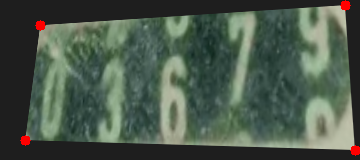
\includegraphics[width=0.95\linewidth]{../assets/tilted.png}\\{\scriptsize simulated angled photo; 4 corners marked (red)}
    \end{center}\end{column}
  \end{columns}
  \vspace{3pt}
  The corners are the correspondences: where each red dot \emph{is} vs where it \emph{should} be.
\end{frame}

\begin{frame}{Step 3--4: warp to a flat scan}
  \begin{columns}[T]
    \begin{column}{0.5\textwidth}\begin{center}
      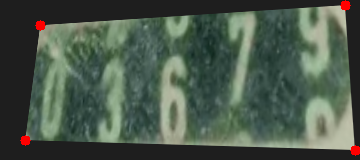
\includegraphics[width=0.95\linewidth]{../assets/tilted.png}\\{\scriptsize input: angled photo}
    \end{center}\end{column}
    \begin{column}{0.5\textwidth}\begin{center}
      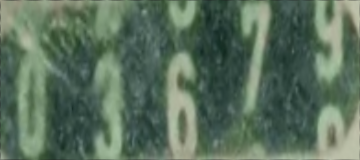
\includegraphics[width=0.95\linewidth]{../assets/recovered.png}\\{\scriptsize output: rectified, front-on}
    \end{center}\end{column}
  \end{columns}
  \vspace{3pt}
  \code{H = getPerspectiveTransform(corners, rectangle)}; \code{warpPerspective(photo, H, size)}. Digits are now readable.
\end{frame}

\begin{frame}{Getting the 4 corners in the right order}
  \begin{itemize}
    \item \code{approxPolyDP} gives 4 points but in \emph{arbitrary} order.
    \item Order them: top-left, top-right, bottom-right, bottom-left — else the warp flips/twists.
    \item Trick: TL has the smallest $x{+}y$; BR the largest; TR the smallest $x{-}y$; BL the largest.
  \end{itemize}
  \begin{badbox}
    Wrong corner order = a mirrored or rotated scan. Always sort the corners consistently.
  \end{badbox}
\end{frame}

\begin{frame}{Worked example: order these 4 corners}
  \begin{columns}[T]
    \begin{column}{0.52\textwidth}
      Detected (arbitrary order):
      \begin{center}
      \begin{tabular}{@{}lrrr@{}}
        \toprule
        Point & $x$ & $y$ & $x{+}y$ \\
        \midrule
        A & 90 & 300 & 390 \\
        B & 120 & 40 & 160 \\
        C & 470 & 360 & 830 \\
        D & 500 & 60 & 560 \\
        \bottomrule
      \end{tabular}
      \end{center}
    \end{column}
    \begin{column}{0.48\textwidth}
      \begin{itemize}
        \item TL = min $x{+}y$ $\Rightarrow$ B.
        \item BR = max $x{+}y$ $\Rightarrow$ C.
        \item Of the rest: TR = min $x{-}y$. $x{-}y$: A$=-210$, D$=440$ $\Rightarrow$ TR = D.
        \item BL = the leftover $\Rightarrow$ A.
      \end{itemize}
      \begin{goodbox}
        Order (B, D, C, A) = (TL, TR, BR, BL).
      \end{goodbox}
    \end{column}
  \end{columns}
\end{frame}

\begin{frame}{Choosing the destination rectangle}
  \begin{itemize}
    \item You are free to pick any clean rectangle; match the object's true aspect ratio.
    \item A4 paper is $1:\sqrt{2}\approx1{:}1.414$. Pick width $W$; height $=W\times1.414$.
    \item A utility meter faceplate might be nearly square, or wider than tall — measure it once.
  \end{itemize}
  \begin{mathbox}
    For $W=800$ and A4: destination $=(0,0),(800,0),(800,1131),(0,1131)$, since $800\times1.414\approx1131$.
  \end{mathbox}
\end{frame}

% ==================================================================
\section{Interpolation \& sampling}
% ==================================================================

\begin{frame}{Inverse warping: every output pixel gets a value}
  \begin{itemize}
    \item \code{warpPerspective} walks the \emph{output} grid, maps each pixel back through $H^{-1}$, and samples the source.
    \item The back-mapped location is almost never an integer — it lands \emph{between} source pixels.
    \item So we must \term{interpolate} a value from the neighbouring source pixels.
  \end{itemize}
  \keyidea{Geometry says \emph{where} to look; interpolation decides the \emph{value} at that fractional spot.}
\end{frame}

\begin{frame}{Interpolation: nearest, bilinear, bicubic}
  \begin{itemize}
    \item \term{Nearest}: copy the closest pixel — blocky but fast; correct for label/mask maps.
    \item \term{Bilinear}: weighted blend of the 4 surrounding pixels — smooth, the sensible default.
    \item \term{Bicubic}: 16-pixel fit — sharper edges, slower; nice for final high-quality output.
  \end{itemize}
  \begin{infobox}
    \code{cv2.INTER\_LINEAR} for photos, \code{INTER\_NEAREST} for segmentation labels, \code{INTER\_CUBIC} for a crisp final scan.
  \end{infobox}
\end{frame}

\begin{frame}{Worked example: bilinear at a fractional point}
  \begin{columns}[T]
    \begin{column}{0.5\textwidth}
      Back-mapped location $(x,y)=(2.25,\,0.75)$ lands inside these four source pixels:
      \begin{center}\pixelgrid{{100,180},{60,220}}\end{center}
      {\scriptsize top-left 100, top-right 180, bottom-left 60, bottom-right 220}
    \end{column}
    \begin{column}{0.5\textwidth}
      \begin{mathbox}
        $a=0.25,\ b=0.75$. Blend along $x$ then $y$:
        \begin{align*}
          \text{top} &= 100(0.75)+180(0.25)=120\\
          \text{bot} &= 60(0.75)+220(0.25)=100\\
          v &= 120(0.25)+100(0.75)=105
        \end{align*}
      \end{mathbox}
      Nearest would have snapped to a single corner (e.g.\ 60) — bilinear gives the smoother 105.
    \end{column}
  \end{columns}
\end{frame}

% ==================================================================
\section{Automatic alignment with RANSAC}
% ==================================================================

\begin{frame}{From matches to a homography}
  \begin{itemize}
    \item Instead of hand-picking 4 corners, use Week 10's feature matches.
    \item But matches contain wrong ones — a plain least-squares fit would be ruined by outliers.
    \item \term{RANSAC}: repeatedly fit $H$ from 4 random matches, keep the $H$ that most matches agree with.
  \end{itemize}
  \begin{mathbox}
    RANSAC = RANdom SAmple Consensus. It finds the transform supported by the largest set of \term{inliers}.
  \end{mathbox}
\end{frame}

\begin{frame}{RANSAC, step by step}
  \begin{enumerate}
    \item Pick 4 random correspondences; compute a candidate $H$.
    \item Count \term{inliers}: matches whose points $H$ maps to within a few pixels.
    \item Repeat many times; keep the $H$ with the most inliers.
    \item Refit $H$ using \emph{all} its inliers for a precise result.
  \end{enumerate}
  \keyidea{RANSAC tolerates a large fraction of wrong matches — it only needs 4 good ones to exist.}
\end{frame}

\begin{frame}{Reprojection error: what ``agree'' means}
  \begin{columns}[T]
    \begin{column}{0.56\textwidth}
      \begin{itemize}
        \item Push each source point through the candidate $H$; compare to its matched point.
        \item Distance below a threshold $\tau$ (say 3 px) $\Rightarrow$ \term{inlier}; else \term{outlier}.
        \item The best $H$ maximises inlier count; \code{ransacReprojThreshold} sets $\tau$.
      \end{itemize}
    \end{column}
    \begin{column}{0.44\textwidth}
      \begin{center}
      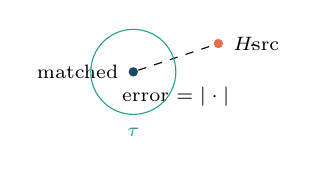
\begin{tikzpicture}[font=\scriptsize,>=Stealth,scale=0.9]
        \node[coursePrimary,circle,fill,inner sep=1.2pt] (m) at (0,0) {};
        \node[left] at (m.west) {matched};
        \node[courseAccent,circle,fill,inner sep=1.2pt] (p) at (1.2,0.4) {};
        \node[right] at (p.east) {$H\!\cdot\!$src};
        \draw[dashed] (m) -- (p);
        \node at (0.6,-0.35) {error $=|\cdot|$};
        \draw[courseGood] (0,0) circle (0.6);
        \node[courseGood] at (0,-0.85) {$\tau$};
      \end{tikzpicture}
      \end{center}
    \end{column}
  \end{columns}
\end{frame}

\begin{frame}{How many iterations? (a quick estimate)}
  \begin{mathbox}
    With inlier fraction $w$ and sample size $s{=}4$, the chance all 4 are inliers is $w^4$.
    To succeed with probability $p$:
    \[ N=\frac{\log(1-p)}{\log(1-w^{4})} \]
  \end{mathbox}
  \begin{itemize}
    \item Example: $w=0.6,\ p=0.99$ $\Rightarrow$ $w^4\approx0.13$, $N\approx\dfrac{\log 0.01}{\log 0.87}\approx 33$ iterations.
    \item Worse matches (smaller $w$) blow up $N$ fast — filter matches first (ratio test) to raise $w$.
  \end{itemize}
\end{frame}

\begin{frame}{Automatic rectification on the real meter}
  \begin{columns}[T]
    \begin{column}{0.5\textwidth}\begin{center}
      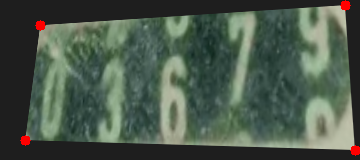
\includegraphics[width=0.95\linewidth]{../assets/tilted.png}\\{\scriptsize angled photo (input)}
    \end{center}\end{column}
    \begin{column}{0.5\textwidth}\begin{center}
      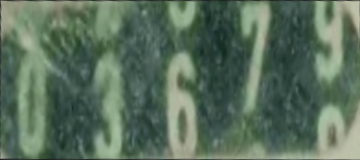
\includegraphics[width=0.95\linewidth]{../assets/auto_rectified.png}\\{\scriptsize auto-rectified via ORB + RANSAC}
    \end{center}\end{column}
  \end{columns}
  \vspace{2pt}
  No manual corners: 66 ORB matches $\rightarrow$ 57 RANSAC inliers $\rightarrow$ \code{findHomography} $\rightarrow$ flat scan.
\end{frame}

% ==================================================================
\section{In-class exercise}
% ==================================================================

\begin{frame}{\faPen~In-class exercise (10 min)}
  \begin{infobox}[Design the rectifier]
  \end{infobox}
  \begin{enumerate}
    \item You have the 4 page corners in the photo. What are the destination points for an
          A4-shaped scan of width 1000?
    \item You resize a segmentation mask through the same warp. Which interpolation, and why?
    \item Your automatic pipeline has 200 feature matches, 60 of them wrong. Which step saves you?
    \item Roughly how many RANSAC iterations for $w=0.7,\ p=0.99$? (order of magnitude is fine)
  \end{enumerate}
\end{frame}

\begin{frame}{\faPen~Debrief}
  \begin{itemize}
    \item (1) $(0,0),(1000,0),(1000,1414),(0,1414)$ — height $=1000\times1.414$.
    \item (2) \code{INTER\_NEAREST}: labels are categorical, blending would invent nonexistent class IDs.
    \item (3) \term{RANSAC} inside \code{findHomography} — it ignores the 60 outliers and fits to the inliers.
    \item (4) $w^4\approx0.24$, $N\approx\log(0.01)/\log(0.76)\approx 17$ — a couple dozen tries.
  \end{itemize}
  \keyidea{Corners (or matches) + destination rectangle + homography + warp = a scanner in four lines of code.}
\end{frame}

% ==================================================================
\section{Deep dive \& limits}
% ==================================================================

\begin{frame}{Planar assumption \& its limits}
  \begin{itemize}
    \item A homography is exact only for a \emph{flat} surface (or a camera that only rotates).
    \item A curved page, a bent meter cover, or 3D objects break the model.
    \item For a gently curved document you need \term{dewarping} (a nonlinear grid) — beyond a single $H$.
  \end{itemize}
  \begin{badbox}
    If your ``scan'' still bows at the edges, the surface wasn't flat — one homography can't fix curvature.
  \end{badbox}
\end{frame}

\begin{frame}{Other uses of homography}
  \begin{itemize}
    \item \term{Panorama stitching}: warp each photo into a common frame and blend.
    \item \term{Augmented reality}: place a graphic onto a detected planar marker.
    \item \term{Bird's-eye view}: rectify a road/parking scene to a top-down map.
    \item \term{DocScan}: our meter/plate rectifier.
  \end{itemize}
  \keyidea{Any time the world of interest is (locally) a plane, a homography is the right tool.}
\end{frame}

\begin{frame}[fragile]{The whole rectifier in code}
\begin{lstlisting}[language=Python]
# corners: 4 page corners found in the photo (ordered TL,TR,BR,BL)
W, H = 800, int(800*1.414)
dst = np.float32([[0,0],[W,0],[W,H],[0,H]])
M = cv2.getPerspectiveTransform(corners, dst)
scan = cv2.warpPerspective(photo, M, (W, H),
                           flags=cv2.INTER_CUBIC)
# automatic variant: ORB matches -> cv2.findHomography(..., cv2.RANSAC)
\end{lstlisting}
  Four lines turn an angled photo into a flat scan — the heart of DocScan.
\end{frame}

\begin{frame}[fragile]{The automatic variant, annotated}
\begin{lstlisting}[language=Python]
orb = cv2.ORB_create(2000)
k1,d1 = orb.detectAndCompute(template, None)
k2,d2 = orb.detectAndCompute(photo, None)
matches = matcher.match(d1, d2)              # some are wrong
src = np.float32([k1[m.queryIdx].pt for m in matches])
dst = np.float32([k2[m.trainIdx].pt for m in matches])
H, mask = cv2.findHomography(dst, src, cv2.RANSAC, 3.0)
print("inliers:", int(mask.sum()), "/", len(matches))
scan = cv2.warpPerspective(photo, H, template.shape[1::-1])
\end{lstlisting}
  \code{mask} flags the inliers; the printed ratio is your confidence the alignment is good.
\end{frame}

% ==================================================================
\section{Pitfalls \& good practice}
% ==================================================================

\begin{frame}{Common pitfalls}
  \begin{badbox}[Too few or degenerate points]
    Three collinear ``corners'' can't define $H$. Ensure the 4 points form a real quadrilateral.
  \end{badbox}
  \begin{badbox}[Loose RANSAC threshold]
    A large $\tau$ lets outliers count as inliers and drags $H$ off. Start around 3 px and tighten.
  \end{badbox}
\end{frame}

\begin{frame}{Good practice}
  \begin{goodbox}[Filter matches before RANSAC]
    A ratio test (Week 10) raises the inlier fraction $w$, which slashes the iterations $N$ needed.
  \end{goodbox}
  \begin{goodbox}[Always report the inlier ratio]
    High inliers/total $\Rightarrow$ trust the scan. A low ratio is your early warning to re-shoot.
  \end{goodbox}
\end{frame}

% ==================================================================
\section{Wrap-up}
% ==================================================================

\begin{frame}{What you should now be able to do}
  \begin{itemize}
    \item Rectify a tilted document: order corners, pick a destination rectangle, build $H$, \code{warpPerspective}.
    \item Choose the right interpolation for photos vs.\ label maps.
    \item Align automatically from feature matches with \code{findHomography} + RANSAC, and read the inlier ratio.
    \item Recognise when the planar assumption breaks and dewarping is needed.
  \end{itemize}
\end{frame}

\begin{frame}{This week's deliverable}
  \begin{alertblock}{Due before Week 12 (see \code{project/})}
    \begin{enumerate}
      \item Take/simulate an angled photo of a meter or document; detect its 4 corners and order them.
      \item Rectify to a flat scan with \code{warpPerspective}; try nearest vs.\ bilinear and compare.
      \item Also rectify automatically via ORB matches + \code{findHomography(RANSAC)}; report inliers/total.
      \item Reflect: after rectification, why is digit reading (Weeks 12--14) much easier?
    \end{enumerate}
  \end{alertblock}
\end{frame}

\begin{frame}[standout]
  A homography turns a snapshot into a scan.\\[4pt]
  \normalsize Four corners, one $3\times3$ matrix, one warp — and the page lies flat.
\end{frame}

\end{document}
